\PassOptionsToPackage{unicode=true}{hyperref} % options for packages loaded elsewhere
\PassOptionsToPackage{hyphens}{url}
%
\documentclass[11,]{article}
\usepackage{lmodern}
\usepackage{amssymb,amsmath}
\usepackage{ifxetex,ifluatex}
\usepackage{caption}
\usepackage{lastpage}
\usepackage{fancyhdr}
\pagestyle{fancy} 
\renewcommand{\headrulewidth}{0pt}
\fancyhead{}
\cfoot{Page \thepage\ of \pageref{LastPage}}
\usepackage{fixltx2e} % provides \textsubscript
\ifnum 0\ifxetex 1\fi\ifluatex 1\fi=0 % if pdftex
  \usepackage[T1]{fontenc}
  \usepackage[utf8]{inputenc}
  \usepackage{textcomp} % provides euro and other symbols
\else % if luatex or xelatex
  \usepackage{unicode-math}
  \defaultfontfeatures{Ligatures=TeX,Scale=MatchLowercase}
\fi
% use upquote if available, for straight quotes in verbatim environments
\IfFileExists{upquote.sty}{\usepackage{upquote}}{}
% use microtype if available
\IfFileExists{microtype.sty}{%
\usepackage[]{microtype}
\UseMicrotypeSet[protrusion]{basicmath} % disable protrusion for tt fonts
}{}
\IfFileExists{parskip.sty}{%
\usepackage{parskip}
}{% else
\setlength{\parindent}{0pt}
\setlength{\parskip}{6pt plus 2pt minus 1pt}
}
\usepackage{hyperref}
\hypersetup{
            pdftitle={Segurança Informática em Redes e Sistemas},
            pdfauthor={Alameda -- Grupo 12},
            pdfborder={0 0 0},
            breaklinks=true}
\urlstyle{same}  % don't use monospace font for urls
\usepackage{graphicx,grffile}
\makeatletter
\def\maxwidth{\ifdim\Gin@nat@width>\linewidth\linewidth\else\Gin@nat@width\fi}
\def\maxheight{\ifdim\Gin@nat@height>\textheight\textheight\else\Gin@nat@height\fi}
\makeatother
% Scale images if necessary, so that they will not overflow the page
% margins by default, and it is still possible to overwrite the defaults
% using explicit options in \includegraphics[width, height, ...]{}
\setkeys{Gin}{width=\maxwidth,height=\maxheight,keepaspectratio}
\setlength{\emergencystretch}{3em}  % prevent overfull lines
\providecommand{\tightlist}{%
  \setlength{\itemsep}{0pt}\setlength{\parskip}{0pt}}
\setcounter{secnumdepth}{0}
% Redefines (sub)paragraphs to behave more like sections
\ifx\paragraph\undefined\else
\let\oldparagraph\paragraph
\renewcommand{\paragraph}[1]{\oldparagraph{#1}\mbox{}}
\fi
\ifx\subparagraph\undefined\else
\let\oldsubparagraph\subparagraph
\renewcommand{\subparagraph}[1]{\oldsubparagraph{#1}\mbox{}}
\fi

% set default figure placement to htbp
\makeatletter
\def\fps@figure{htbp}
\makeatother


\title{Segurança Informática em Redes e Sistemas}
\author{Alameda -- Grupo 12}
\date{}

\begin{document}
\maketitle

\begin{figure}
\centering
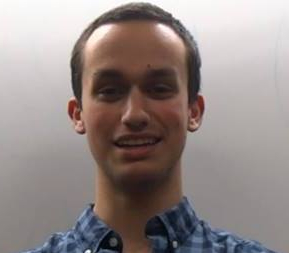
\includegraphics[width=0.3\textwidth,height=\textheight]{81201.jpg}
\captionsetup{labelformat=empty}
\caption{81201 -- Tomás Cunha -- tomas.cunha@tecnico.ulisboa.pt}
\end{figure}

\begin{figure}
\centering

\includegraphics[width=0.3\textwidth,height=\textheight]{81209.jpg}
\captionsetup{labelformat=empty}
\caption{81209 -- Guilherme Santos --
guilherme.j.santos@tecnico.ulisboa.pt}
\end{figure}

\begin{figure}
\centering

\includegraphics[width=0.3\textwidth,height=\textheight]{81703.jpg}
\captionsetup{labelformat=empty}
\caption{81703 -- Nuno Santos -- nuno.v.santos@tecnico.ulisboa.pt}
\end{figure}

\newpage

\hypertarget{problem}{%
\section{Problem}\label{problem}}

After pairing the phone with the computer, keys are generated and
certain files on the computer can be encrypted when the phone is not
connected to it. A phone is connected when near to the computer through
the exchange of a token.

We need to ensure that:

\begin{itemize}
\item
  the paired computer files can only be decrypted with the paired
  phone's presence, so attackers can't fake the phone's presence.
\item
  the phone only sends the token to the paired computer, so attackers
  can't fake the computer's presence. Otherwise the fake computer can
  get the token and use a fake phone to decrypt the files.
\item
  the key exchange (token) is secure because if the attacker is
  listening and gets the exchanged message by the phone he cannot get
  the keys to decrypt the files.
\item
  token needs to be unique to avoid replay attacks.
\item
  the key storage needs to be secure so that if the device keeping the
  keys is compromised the attacker cannot get the keys to decrypt the
  files.
\end{itemize}

\begin{description}
\item[Problem being solved:]
Only those with access to both the paired phone and computer can access
the encrypted files.
\end{description}

\hypertarget{requirements}{%
\section{Requirements}\label{requirements}}

\begin{enumerate}
\tightlist
\item
  Confidentiality (only the paired computer can read the token)
\item
  Authentication of origin (the paired computer only accepts tokens sent
  by the paired phone)
\item
  Fault tolerance (if the computer crashes when the computer is
  connected, the files cannot be left unprotected)
\end{enumerate}

\hypertarget{solution}{%
\section{Solution}\label{solution}}

During the initial pairing, the PC creates and displays its RSA public
key in a QR code on the screen. The phone scans this key and stores it.
Then, it generates and sends an AES-256 session key and sends it
encrypted with the PC's public key. Afterwards, using that key for
encrypting the traffic, it sends its own public key, which is stored by
the PC to be used as a Key Encryption Key. This serves as a protection
from man-in-the-middle attacks.

The phone generates two other AES-256 keys, one to be used for file
encryption, and one to encrypt that key before sending it to the PC.
This key is stored, and the pairing process is completed.

After pairing, the phone can connect to the PC, who (after the initial
session key exchange) sends the encrypted File Encryption key, which is
securely stored on the PC. The phone decrypts it and sends it back to
the PC, who uses it to decrypt the files. The phone then has to keep
sending heartbeats (which include a nonce to avoid replay attacks) so
that the PC can know the phone is in range. After the phone is
disconnected, since the PC no longer receives heartbeats, it encrypts
the files again and deletes the FE key from storage, keeping only its
encrypted copy. The PC maintains a log of the operations it performs. In
case of a crash, after recovery it will encrypt all the files with the
decrypted FE key, then deletes the key and waits for the phone to be
reconnected.

See figure \ref{sol_diagram} for information.

\begin{description}
\item[Basic]
Initial implementation without fault tolerance and secure channels.
\item[Intermediate]
Implementation of confidentiality with secure channels.
\item[Advanced]
Implementation of fault tolerance.
\end{description}

\hypertarget{results}{%
\section{Results}\label{results}}

The entirety of the proposed solution was implemented in separate
Android and Python applications. It was thoroughly tested and
successfully recovered from faults, and files were successfully
encrypted and decrypted while the phone was in range/out of range
(respectively).

All encrypted data (except for any session key exchanges, which use
RSA-OAEP with 2048 bit keys) is encrypted using AES-256 in EAX mode.

The architecture that was used is described in the annexed figure
\ref{uml}.

\hypertarget{evaluation}{%
\section{Evaluation}\label{evaluation}}

Although the application itself is secure, it assumes a certain level of
responsibility on the user's side. The user needs to remember at least
one password, if they use the same password on the phone and the PC
(which is not the recommended way to do it), or potentially two
passwords, if they choose to be cautious and use different passwords for
both devices. If either of these passwords is forgotten, the files are
irrecoverably lost.

It is also vulnerable to an attacker that gains access to the
configuration folder and its contained files. Although that attacker
can't retrieve the keys from these files alone without knowing the
password, they can delete the files, resulting in the user losing their
keys. This can be mitigated by keeping backups of the configuration
folder whenever it gets modified, however.

If the attacker manages to crash the program while the files are
encrypted, they are left in a vulnerable state until the program is
restarted and the password is inputted. They are immediately
re-encrypted as soon as the program is restarted, however, which is good
enough for the general case where the user's PC might crash while the
program is running and they want to make sure the files are protected
when the PC gets turned back on. We consider that if the attacker has
access to the computer while the files are decrypted, they can already
copy the files anyway, so this is beyond the scope of the application.

Finally, the attacker might jam the Bluetooth connection and prevent the
computer from receiving any messages from the phone. This would result
in the computer being unable to decrypt the files (\textbf{Denial of
Service} attack).

Besides these vulnerabilities, the application ensures, as said in the
\protect\hyperlink{requirements}{\textbf{requirements}} section,
confidentiality, authenticity, and fault tolerance:

\begin{itemize}
\tightlist
\item
  It is protected from replay attacks, since heartbeats carry nonces
\item
  The session is always encrypted and authenticated using AES EAX mode,
  so the attacker can't tamper with heartbeats to fake a new nonce.
\item
  Every configuration file is encrypted using the user's password (which
  may be different on each device), so even if an attacker manages to
  get these files, they can't get the keys.
\end{itemize}

\hypertarget{conclusion}{%
\section{Conclusion}\label{conclusion}}

Overall, the project was implemented as expected. Although it doesn't
have the best interface, which is not within the scope of this course,
it fulfills its purpose successfully and securely.

Achieving interoperability between the two different environments was
challenging, but it allowed us to learn more.

\hypertarget{references}{%
\section{References}\label{references}}

\hypertarget{tools-used}{%
\subsection{Tools used}\label{tools-used}}

\begin{itemize}
\tightlist
\item
  Git
\item
  Java 8

  \begin{itemize}
  \tightlist
  \item
    Android Studio
  \end{itemize}
\item
  Python 3.6

  \begin{itemize}
  \tightlist
  \item
    PyCharm
  \end{itemize}
\end{itemize}

\hypertarget{libraries-used}{%
\subsection{Libraries used}\label{libraries-used}}

\hypertarget{python}{%
\subsubsection{Python}\label{python}}

\begin{itemize}
\tightlist
\item
  qrcode
\item
  typing
\item
  pybluez
\item
  pyyaml
\item
  pypubsub
\item
  pycryptodomex
\item
  appdirs
\end{itemize}

\hypertarget{java}{%
\subsubsection{Java}\label{java}}

\begin{itemize}
\tightlist
\item
  spongycastle
\item
  zxing
\end{itemize}

\newpage

\hypertarget{annex}{%
\section{Annex}\label{annex}}

\begin{figure}
\centering
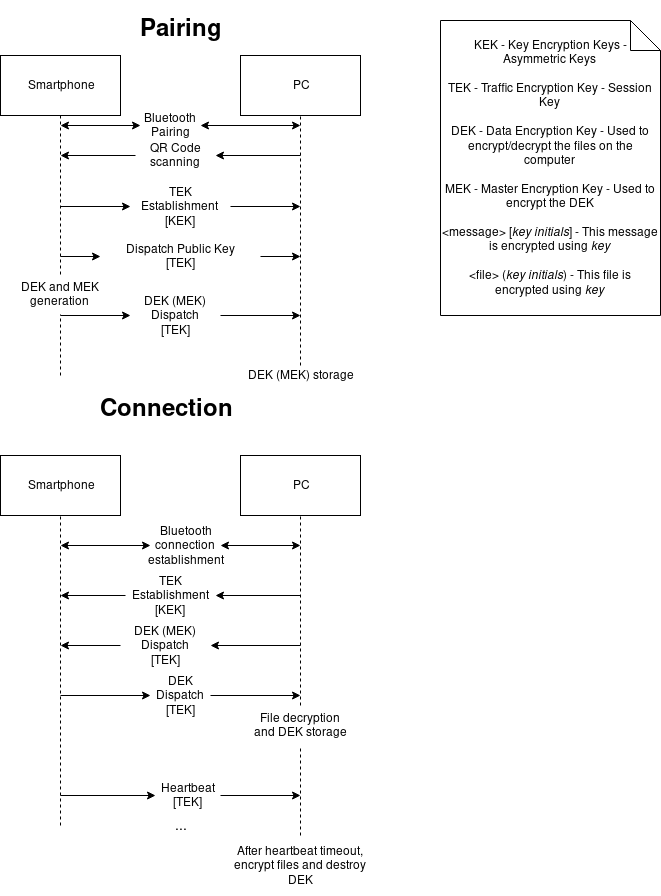
\includegraphics[width=\textwidth,height=1\textwidth]{Solution_Diagram.png}
\caption{Communication diagram on the proposed
solution\label{sol_diagram}}
\end{figure}

\begin{figure}
\centering
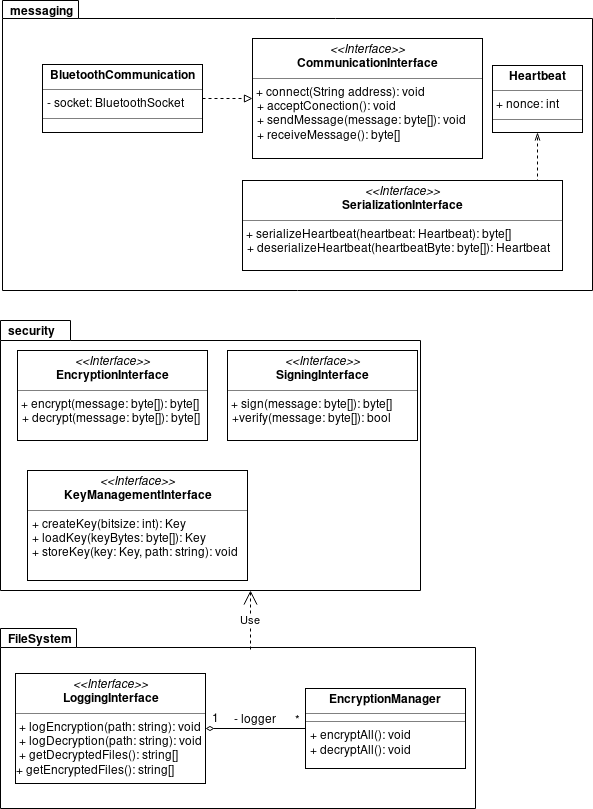
\includegraphics[width=\textwidth,height=1\textwidth]{SIRS_Packages.png}
\caption{Project Class Diagram -- The application then had a UI Module
and an Application singleton that invoked the methods on these
objects\label{uml}}
\end{figure}

\end{document}
